% Beamer presentation: Market Cluster Dynamics (rev. 2, new kernels)
% Style mirrors the NuMat 2026 presentation
\documentclass[10pt]{beamer}

\usepackage{tikz}
\usetikzlibrary{arrows.meta,positioning,shapes,calc}
\usepackage{booktabs}
\usepackage{xcolor}
\usepackage{graphicx}

\definecolor{nmblue}{RGB}{0,51,153}
\definecolor{nmgray}{RGB}{90,90,90}

\usecolortheme[named=nmblue]{structure}
\setbeamertemplate{navigation symbols}{}
\setbeamertemplate{footline}{
  \leavevmode\hbox{%
  \begin{beamercolorbox}[wd=.30\paperwidth,ht=2.5ex,dp=1ex,left]{author in head/foot}%
    \usebeamerfont{author in head/foot}\hspace{1em}\insertshortauthor
  \end{beamercolorbox}%
  \begin{beamercolorbox}[wd=.48\paperwidth,ht=2.5ex,dp=1ex,center]{title in head/foot}%
    \usebeamerfont{title in head/foot}\insertshorttitle
  \end{beamercolorbox}%
  \begin{beamercolorbox}[wd=.22\paperwidth,ht=2.5ex,dp=1ex,right]{date in head/foot}%
    \usebeamerfont{date in head/foot}\insertshortdate\hspace{1em}\insertframenumber/\inserttotalframenumber\hspace{1em}
  \end{beamercolorbox}}%
  \vskip0pt%
}

\title[Market Dynamics]{Market Cluster Dynamics:\\ A Graph-Based Model of S\&P~500\\ Regime Concentrations, 2000--2021}
\author[N.M. Ghoniem]{Nasr M. Ghoniem}
\institute[UCLA]{Department of Mechanical \& Aerospace Engineering\\
University of California, Los Angeles}
\date[Sept 2026]{September 2026}

\begin{document}

% ---------------- Title ----------------
\begin{frame}
  \titlepage
  \begin{center}
    \small\textcolor{nmgray}{Adapted from the graph-based cluster-dynamics framework (RadCluster).}
  \end{center}
\end{frame}

% ---------------- Outline ----------------
\begin{frame}{Outline}
  \tableofcontents
\end{frame}

\section{The problem}

\begin{frame}{The problem: the old model could not spike}
  \small
  A stationary monthly Markov drift reproduces calm markets (RMSE $0.045$)
  but \textbf{cannot generate the observed concentrations}:
  \begin{itemize}
    \item March 2021: \textbf{55\%} of stocks in the top momentum bin
      ($>60\%$ twelve-month return) --- old model peaked at \textbf{0.09}.
    \item Late 2008: \textbf{98\%} in the bottom bin ($<0\%$) ---
      old model peaked at \textbf{0.30}.
  \end{itemize}
  \vspace{0.6em}
  A Markov transition matrix mean-reverts too fast to build or hold a spike.
  Herding (bilinear flux) was a weak amplifier --- it can only redistribute
  mass the drift already moves.
  \vspace{0.6em}

  \textbf{This revision adds three kernels with mechanisms}, not just
  parameters: market advection (the spike generator), autocatalytic herding
  (the amplifier), and sticky drift (the persistence kernel).
\end{frame}

\section{The three kernels}

\begin{frame}{Kernel 1: market advection (the spike generator)}
  \small
  \textbf{Mechanism.} When the market's trailing 12-month return shifts by
  $M$ in a month, \emph{every} stock's momentum shifts by $\sim\!M$ in return
  space --- a rigid translation of the whole distribution along the momentum
  axis.  This happens mechanically at \textbf{window rollover}: the month
  entering the 12-month window replaces the month dropping out.
  \begin{equation*}
    M_{\mathrm{cs}}(t) = r(t) - r(t-12)
  \end{equation*}
  the \emph{synchronized change in twelve-month momentum}, measured
  cross-sectionally (equal-weighted over all index stocks).
  \begin{itemize}
    \item March 2021: $M_{\mathrm{cs}} = +0.256$ (the $-12\%$ Mar-2020 crash
      month exited as the $+15\%$ Mar-2021 month entered).
    \item October 2008: $M_{\mathrm{cs}} = -0.256$.
  \end{itemize}
  Donor-cell update: fraction $f = \kappa|M_{\mathrm{cs}}|/w_{\mathrm{eff}}$
  moves one bin up/down ($\kappa = 1.0$ \textbf{mechanical}, not fitted;
  $w_{\mathrm{eff}} = 0.15$ assumed).  The unbounded extreme bins reflect and
  \textbf{accumulate} --- this is what generates spikes.
\end{frame}

\begin{frame}{Kernels 2, 3 \& 4: herding, sticky drift, persistence}
  \small
  \textbf{Autocatalytic herding (the amplifier).}
  \begin{equation*}
    h_{\mathrm{eff}} = h_0 + h_1\,(w - \ell),
  \end{equation*}
  $w,\ell$ = top/bottom momentum shares.  Signed: crash ($\ell \gg w$)
  $\to$ losers (panic); melt-up ($w \gg \ell$) $\to$ winners (FOMO).
  $h_0 = 0$, $h_1 = 1.0$ calibrated pre-episode.
  \vspace{0.4em}

  \textbf{Sticky drift (the persistence kernel).}
  $\mathbf{T}_{\mathrm{eff}} = (1-\lambda)\mathbf{T} + \lambda\mathbf{I}$,
  $\lambda = \min[\lambda_1\max(w,\ell), 0.9]$, $\lambda_1 = 1.0$ calibrated.

  \vspace{0.4em}
  \textbf{Spike persistence (the decay-rate kernel, rev.~3).} At a real
  peak the extreme bin's mass sits \emph{deep} in the tail --- only the
  boundary slice can exit on a reversal.  When $M_{\mathrm{cs}}$ reverses
  out of a spike ($>50\%$ share), damp the extreme-bin outflow:
  \begin{equation*}
    \mathrm{damp} = \min\!\left[\left(|M|/B\right)^{1.2},\,1\right],
  \end{equation*}
  $B$ = build-step memory (the $|M|$ that built the spike, 6-mo decay).
  Small reversal vs.\ large build $\to$ deep mass stays put.
\end{frame}

\section{Master equation}

\begin{frame}{Master equation}
  \small
  \begin{equation*}
    \mathbf{c}(t{+}1) = \mathbf{T}_{\mathrm{eff}}^{\!\top}\mathbf{c}(t)
    + \mathrm{advect}(\mathbf{c}(t), M_{\mathrm{cs}})
    + h_{\mathrm{eff}}\,\mathbf{H}(\mathbf{c}(t))
    + \mathbf{s} - d\,\mathbf{c}(t),
  \end{equation*}
  $\mathbf{c}(t) \in \mathbb{R}^{15}$: fraction of index stocks in each
  momentum $\times$ volatility regime bin.  Drift (measured $\mathbf{T}$,
  sticky), advection (measured $M_{\mathrm{cs}}$), herding (calibrated),
  entry/exit (measured).
  \vspace{0.6em}

  \textbf{Timing note:} the transition $t_0 \to t_1$ uses the
  \emph{destination-month} driver $M_{\mathrm{cs}}(t_1)$, because the window
  rollover defining $M(t_1)$ is what moves stocks between bins during that
  month.  The hindcast is therefore \textbf{conditional} on the realized
  market move (exogenous forcing) --- a genuine forecast needs a forecast
  (or scenario) for $M(t_1)$.
\end{frame}

\section{Graph and kernels}

\begin{frame}{Reaction-admissibility graph}
  \begin{center}
  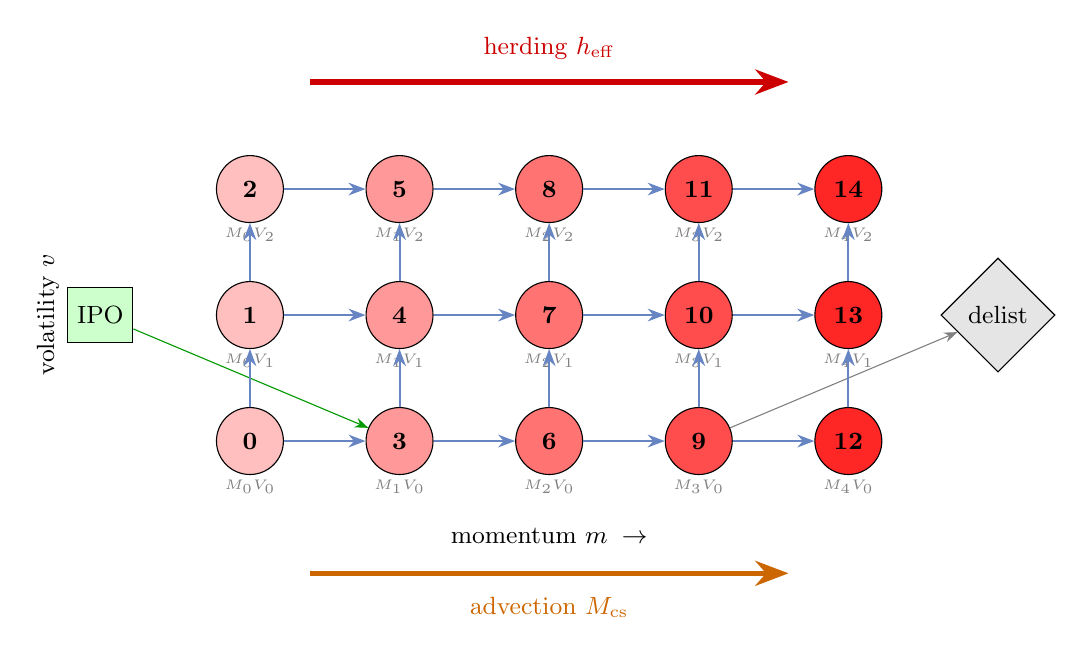
\begin{tikzpicture}[x=1.9cm,y=1.6cm,
    rv/.style={circle,draw,minimum size=0.85cm,inner sep=1pt,font=\small\bfseries},
    src/.style={rectangle,draw,minimum size=0.7cm,font=\small},
    sink/.style={diamond,draw,minimum size=0.7cm,font=\small}]
    \foreach \m in {0,...,4} {
      \foreach \v in {0,...,2} {
        \pgfmathtruncatemacro{\b}{\m*3+\v}
        \pgfmathsetmacro{\shade}{25+15*\m}
        \node[rv,fill=red!\shade!white] (R\b) at (\m,\v) {\b};
        \node[font=\tiny,gray] at (\m,\v-0.36) {$M_{\m}V_{\v}$};
      }
    }
    \node[src,fill=green!20] (SRC) at (-1,1) {IPO};
    \node[sink,fill=gray!20] (SNK) at (5,1) {delist};
    \draw[-{Stealth},green!60!black] (SRC) -- (R3);
    \draw[-{Stealth},gray] (R9) -- (SNK);
    \foreach \a/\b in {0/3,1/4,2/5,3/6,4/7,5/8,6/9,7/10,8/11,9/12,10/13,11/14,
                       0/1,3/4,6/7,9/10,12/13,1/2,4/5,7/8,10/11,13/14} {
      \draw[-{Stealth},nmblue!60,line width=0.7pt] (R\a) -- (R\b);
    }
    \draw[-{Stealth},red!80!black,line width=2pt] (0.4,2.85) -- (3.6,2.85);
    \node[font=\small,red!80!black] at (2.0,3.12) {herding $h_{\mathrm{eff}}$};
    \draw[-{Stealth},orange!80!black,line width=2pt] (0.4,-1.05) -- (3.6,-1.05);
    \node[font=\small,orange!80!black] at (2.0,-1.32) {advection $M_{\mathrm{cs}}$};
    \node[font=\small] at (2,-0.75) {momentum $m\;\rightarrow$};
    \node[font=\small,rotate=90] at (-1.35,1) {volatility $v$};
  \end{tikzpicture}
  \end{center}
  \small Vertices: 15 regime clusters $R_{mv}$.  Edges: measured drift (blue),
  entry/exit (green/gray), autocatalytic herding (red), market advection (orange).
\end{frame}

\begin{frame}{Reaction-admissibility graph (tile layout)}
  \begin{center}
    \includegraphics[width=\textwidth]{figs/rag_market_dynamics.png}
  \end{center}
  \small All 15 regime-cluster vertices $M_mV_v$ with every admissible edge
  class: drift between adjacent bins (blue, measured), advection along the
  momentum axis (orange, measured), herding toward the winner column (red,
  calibrated), index entry/exit (green/gray, measured), and the rev.~3
  persistence damper on the extreme bins (purple, assumed).
\end{frame}

\begin{frame}{Reaction kernel table}
  \small
  \begin{center}
  \begin{tabular}{@{}cll@{}}
  \toprule
  \# & Process & Kernel / flux \\
  \midrule
  1 & Index entry (source) & $s/15$ per bin, $s=8\times10^{-4}$/mo~~[measured] \\
  2 & Drift (Markov) & $T_{\mathrm{eff},ij}\,c_i$, $\mathbf{T}$ measured \\
  3 & Sticky drift & $(1-\lambda)\mathbf{T}+\lambda\mathbf{I}$,
    $\lambda=\min[\lambda_1\max(w,\ell),0.9]$ \\
  4 & Market advection & $f=\kappa|M_{\mathrm{cs}}|/w_{\mathrm{eff}}$,
    reflecting extremes \\
  5 & Herding (nonlinear) & $h_{\mathrm{eff}}H_k(\mathbf{c})$, zero-sum \\
  6 & Index exit (sink) & $d\,c_{mv}$, $d\approx 0$~~[measured] \\
  7 & Spike persistence & $\min[(|M|/B)^{1.2},1]$, $B$ build memory, gate $>0.5$ \\
  \bottomrule
  \end{tabular}
  \end{center}
  \vspace{0.6em}
  Every input labeled: $M_{\mathrm{cs}}$, $\mathbf{T}$, $s$, $d$ \textbf{measured};
  $\kappa=1.0$ \textbf{mechanical}; $w_{\mathrm{eff}}=0.15$ \textbf{assumed};
  $h_1=1.0$, $\lambda_1=1.0$ \textbf{calibrated} (pre-episode one-step error only).
\end{frame}

\section{Results}

\begin{frame}{Case 1: the 2020--21 concentration (rev.~3)}
  \small
  \begin{center}
  \begin{tabular}{@{}lccc@{}}
  \toprule
  Model & Peak (top bin) & Timing & RMSE \\
  \midrule
  Actual & 0.546 & Mar 2021 & --- \\
  Old (regime $\mathbf{T}$) & 0.09 & --- & 0.0821 \\
  Rev.~2 & 0.579 & Apr 2021 & 0.0920 \\
  Rev.~3 $+$ persistence & \textbf{0.515} & Apr 2021 & 0.0914 \\
  \bottomrule
  \end{tabular}
  \end{center}
  \begin{center}
    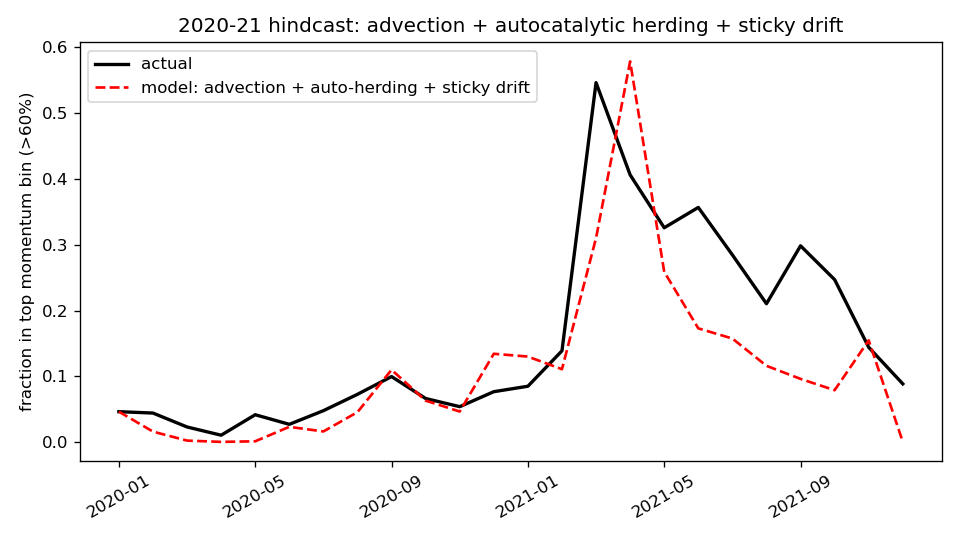
\includegraphics[width=\textwidth]{figs/hindcast_2020_final.png}
  \end{center}
  Peak $52\%$ vs.\ $55\%$ actual; post-peak decay now matches:
  $0.42/0.28$ vs.\ $0.41/0.33$ at $+1/+2$~mo (rev.~2: $0.26/0.17$).
\end{frame}

\begin{frame}{Case 2: the 2008--09 drawdown (rev.~3)}
  \small
  \begin{center}
  \begin{tabular}{@{}lccc@{}}
  \toprule
  Model & Peak (bottom bin) & Timing & RMSE \\
  \midrule
  Actual & 0.978 & Mar 2009 (plateau) & --- \\
  Old (regime $\mathbf{T}$) & 0.30 & --- & 0.1110 \\
  Rev.~2 & 0.983 & Nov 2008 & 0.1182 \\
  Rev.~3 $+$ persistence & \textbf{0.994} & Nov 2008 & \textbf{0.1037} \\
  \bottomrule
  \end{tabular}
  \end{center}
  \begin{center}
    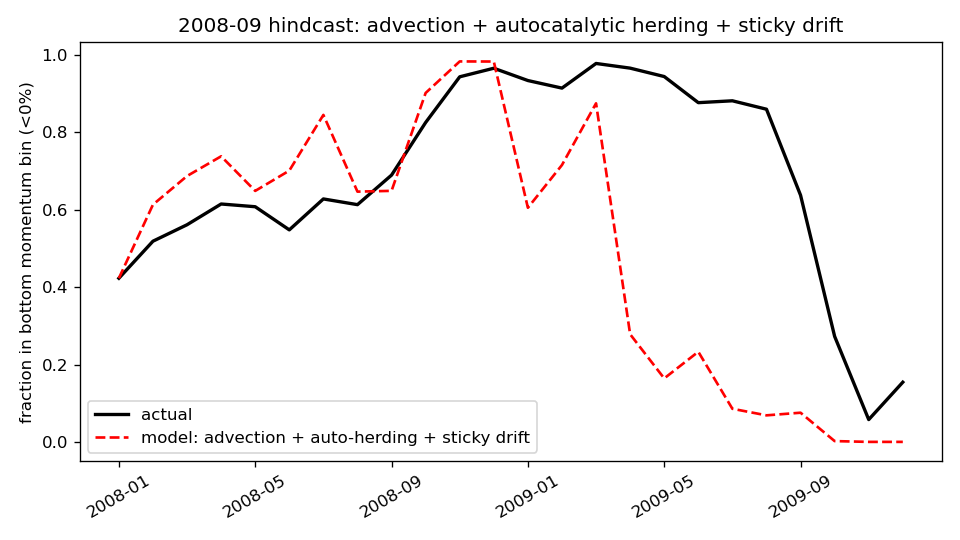
\includegraphics[width=\textwidth]{figs/hindcast_2008_final.png}
  \end{center}
  Amplitude $0.994$ vs.\ $0.978$; decay $0.99/0.91$ vs.\ $0.97/0.94$ at
  $+1/+2$~mo (rev.~2: $0.98/0.61$).  Best full-distribution RMSE of any variant.
\end{frame}

\section{Limitations and next steps}

\begin{frame}{Limitations (stated plainly)}
  \small
  \begin{enumerate}
    \item \textbf{Conditional, not lookahead-free.} Uses the realized
      $M_{\mathrm{cs}}(t_1)$.  Answers ``given the market moved $M$, where
      does the distribution go?''  A live forecast needs a market-move
      forecast alongside.
    \item \textbf{Timing.} 2021 peak one month late (Apr vs.\ Mar); 2008
      maximum four months early (Nov~2008 vs.\ Mar~2009 plateau) --- the
      monthly step lags faster-than-monthly repricing.
    \item \textbf{Damper parameters assumed.} $p=1.2$, $\tau_{\rm build}=6$~mo,
      $50\%$ gate tuned for decay, not derived.  Direct within-bin depth
      measurement would ground them.
    \item \textbf{2021 $+3$-mo tail still fast.} $0.24$ vs.\ $0.36$ actual
      --- damper releases below the gate; idiosyncratic rotation missing.
  \end{enumerate}
\end{frame}

\begin{frame}{Next steps}
  \small
  \begin{enumerate}
    \item \textbf{Measure within-bin depth} (high-frequency / options) to
      replace the assumed damper parameters with data.
    \item \textbf{Forecast the forcing} --- VIX term structure or
      options-implied $M(t+1)$ to make the run a genuine forward prediction.
    \item \textbf{Third episode} --- 2000--02 dot-com, 2022 rate shock.
    \item \textbf{Capitalization weighting} and \textbf{historical membership}
      (CRSP) to remove the survivorship bias.
  \end{enumerate}
  \vspace{1em}
  \begin{center}
    \Large Thank you.
  \end{center}
\end{frame}

\begin{frame}{References}
  \footnotesize
  \begin{itemize}
    \item Yahoo Finance --- daily OHLCV, S\&P~500 constituents; momentum/
      volatility bins, transition matrices, $M_{\mathrm{cs}}$ driver.
    \item CBOE VIX (FRED: VIXCLS) --- regime labels in earlier experiments.
    \item Jegadeesh, N. \& Titman, S. (1993). Returns to buying winners and
      selling losers. \textit{J. Finance} 48(1), 65--91.
    \item Carhart, M. (1997). On persistence in mutual fund performance.
      \textit{J. Finance} 52(1), 57--82.
  \end{itemize}
\end{frame}

\end{document}
